\documentclass[a4paper]{cmspaper} %USE for CMS machines

\usepackage{amsmath}
\usepackage{subfigure}
\usepackage{xspace}

% $ Id: $

% Required pacakges
\usepackage{amsmath}
\usepackage{cancel}
\usepackage{xspace}

\newcommand{\fixme}[1]{\textcolor{red}{{\textbf{FIXME: }\textit{#1}}}}

% Sectioning
\newcommand{\qsec}[1]{Section~\ref{#1}}
\newcommand{\qfig}[1]{Fig.~\ref{#1}}
\newcommand{\qtab}[1]{Table~\ref{#1}}
\newcommand{\qeq}[1]{\eqref{#1}}

% Units
\newcommand{\tev}{\ensuremath{\;\text{Te}\kern-0.06667em\text{V}}\xspace}
\newcommand{\gev}{\ensuremath{\;\text{Ge}\kern-0.06667em\text{V}}\xspace}
\newcommand{\mev}{\ensuremath{\;\text{Me}\kern-0.06667em\text{V}}\xspace}
\newcommand{\km}{\ensuremath{\;\text{km}}\xspace}
\newcommand{\m}{\ensuremath{\;\text{m}}\xspace}
\newcommand{\cm}{\ensuremath{\;\text{cm}}\xspace}
\newcommand{\mm}{\ensuremath{\;\text{mm}}\xspace}
\newcommand{\second}{\ensuremath{\;\text{s}}\xspace}
\newcommand{\tons}{\ensuremath{\;\text{t}}\xspace}
\newcommand{\tesla}{\ensuremath{\;\text{T}}\xspace}
\newcommand{\kelvin}{\ensuremath{\;\text{K}}\xspace}
\newcommand{\pbinv}{\ensuremath{\;\text{pb}^{-1}}\xspace}

% Quantities
\newcommand{\et}{\ensuremath{E_{\text{T}}}\xspace}
\newcommand{\met}{\ensuremath{\slash\mkern-12mu{E}_{\text{T}}}\xspace}
\newcommand{\mht}{\ensuremath{\slash\mkern-12mu{H}_{\text{T}}}\xspace}
\newcommand{\metvec}{\ensuremath{\slash\mkern-12mu{\vec{E}}_{\text{T}}}\xspace}
\newcommand{\pt}{\ensuremath{p_{\text{T}}}\xspace}
\newcommand{\pti}[1]{\ensuremath{p_{\text{T},#1}}\xspace}
\newcommand{\ptvec}{\ensuremath{\vec{p}_{\text{T}}}\xspace}
\newcommand{\ptsub}[1]{\ensuremath{p_{\text{T},#1}}\xspace}
\newcommand{\ptvecsub}[1]{\ensuremath{\vec{p}_{\text{T},#1}}\xspace}
\newcommand{\ptave}{\ensuremath{p^{\text{dijet}}_{\text{T}}}\xspace}
\newcommand{\ptgen}{\ensuremath{p^{\text{gen}}_{\text{T}}}\xspace}
\newcommand{\pthat}{\ensuremath{\hat{p}_{\text{T}}}\xspace}
\newcommand{\pttrue}{\ensuremath{p^{\text{true}}_{\text{T}}}\xspace}
\newcommand{\pttruehigh}[1]{\ensuremath{p^{\text{true,#1}}_{\text{T}}}\xspace}
\newcommand{\ptrel}{\ensuremath{p^{\text{rel}}_{\text{T},3}}\xspace}
\newcommand{\ptcalo}{\ensuremath{p^{\text{calo}}_{\text{T}}}\xspace}
\newcommand{\ptcaloi}[1]{\ensuremath{p^{\text{calo}}_{\text{T},#1}}\xspace}
\newcommand{\ptmin}{\ensuremath{\pt^{\text{min}}}\xspace}
\newcommand{\ptmax}{\ensuremath{\pt^{\text{max}}}\xspace}
\newcommand{\ptreco}{\ensuremath{\pt(\text{reco})}\xspace}
\newcommand{\pp}{\ensuremath{p_{||}}\xspace}
\newcommand{\ppi}[1]{\ensuremath{p_{||,#1}}\xspace}

% Symbols
\newcommand{\dif}[1]{\ensuremath{\text{d}#1}\xspace}
\newcommand{\e}{\,\text{e}}
\newcommand{\nup}[1]{$^{\text{\scriptsize #1}}$}
\newcommand{\dgr}{\ensuremath{\,^{\circ}}}
\newcommand{\mean}[1]{\ensuremath{\langle#1\rangle}}
\newcommand{\gqq}[1]{\ensuremath{\glqq#1\grqq}}
\newcommand{\rarr}{\ensuremath{\rightarrow}\xspace}

% Words and characters
\newcommand{\diagonalsout}[1]{\ensuremath{\cancel{\text{#1}}}}
\newcommand{\genjet}{GenJet\xspace}
\newcommand{\genjets}{GenJets\xspace}
\newcommand{\calojet}{CaloJet\xspace}
\newcommand{\calojets}{CaloJets\xspace}

 %use on CMS machines
\newcommand{\mess}{\ensuremath{p^{\text{meas}}_{\mathrm{T}}}\xspace}
\newcommand{\meas}[1]{\ensuremath{p^{\text{meas}}_{\mathrm{T},#1}}\xspace}
\newcommand{\truth}{\ensuremath{\pt^{\text{true}}}\xspace}
\newcommand{\ptmin}{\ensuremath{\pt^{\text{min}}}\xspace}
\newcommand{\ptmax}{\ensuremath{\pt^{\text{max}}}\xspace}

% pdflatex packages
\usepackage[pdftex]{color,graphicx}
\usepackage[pdftex]{hyperref}
\hypersetup{unicode=true}
\hypersetup{bookmarks=true}
\hypersetup{pdftitle={Determination of the jet energy resolution in QCD dijet events}}
\hypersetup{pdfauthor={Matthias Schr\"oder}}
\hypersetup{colorlinks=false}

\begin{document}

\begin{titlepage}
  \date{\today}
  \title{Determination of the jet energy resolution in QCD dijet
    events using an unbinned maximum likelihood method}
\end{titlepage}

\section{Introduction}
In the following studies on the determination of the jet energy resolution from QCD dijet events are presented in the following.
QCD events have a large cross section e.g. in comparison to $\gamma$-jet events and hence provide a higher \pt reach and an early sensitivity also to non-Gaussian tails of the resolution.

The underlying assumption of this method is the presence of
ideal dijet events.
There are exactly two jets assumed in the event whose true transverse momenta are
balanced.
Their measured transverse momenta are assumed to be
independently affected by the detector resolution.
Here, calorimeter jets are considered i.e. fluctuations of the
measured \pt w.r.t. the true \pt are regarded as an effect of the calorimeter measurement.

A likelihood is constructed from these assumptions.
The constituent probability densities of the dijet events contain a
description of the jet energy resolution.
A suitable parameterisation of the resolution allows description of
non-Gaussian tails.
Moreover, it is possible to include other event types -- such as
$\gamma+$jet events -- into the likelihood, providing the definition
of a proper probability density for these events.


\section{Technique}
\subsection{Discussion of the basic technique}
The underlying assumptions listed above of the presented method are
\begin{itemize}
\item an ideal dijet event configuration with exactly two jets of the
  same true transverse momentum, \truth;
\item measured jet transverse momenta, \meas{i}, resulting from
  independent fluctuations of the calorimeter measurement.
\end{itemize}
% \begin{figure}[ht]
%   \begin{center}
%     \includegraphics[width=0.4\textwidth]{../figures/FlowChartResolutionFit}
%   \end{center}
%   \caption{Sketch of the resolutin fit technique.}
%   \label{fig:resFit:sketchMethod}
% \end{figure}
Based on these, the probability density, \textit{pdf}, of a measured
dijet event configuration is defined as
\begin{equation}
  \label{eq:resFit:dijetPdf}
  f_{\vec{b}}\left(\meas{1},\meas{2}\right) = \int^{t_{1}}_{t_{0}}\dif{\truth}\,f\left(\truth\right)
  \cdot f_{\vec{b}}\left(\meas{1}|\truth\right)
  \cdot f_{\vec{b}}\left(\meas{2}|\truth\right),
\end{equation}
with
\begin{itemize}
\item $f(\truth)$, the pdf of the true \pt in the dijet event i.e. the
  spectrum and
\item $f_{\vec{b}}(\meas{i}|\truth)$, the pdf of the measured \pt
  of the $i$-th jet.
\end{itemize}
It is important to note that knowledge of \truth is not required as it
is integrated out.
However, the pdfs $f(\truth)$ and $f_{\vec{b}}(\meas{i}|\truth)$ have
to be provided.
In the following, the spectrum $f(\truth)$ is assumed to be known
(comp. Sec~/ref{bla}) while $f_{\vec{b}}(\meas{i}|\truth)$ is
parameterised in an apropriate way using the parameter set $\vec{b}$.

If $f(\truth)$ and
$f_{\vec{b}}(\meas{i}|\truth)$ are properly normalised such
that
\begin{eqnarray*}
  1 & = & \int^{t_{1}}_{t_{0}}\dif{\truth}\,f\left(\truth\right) \\
  1 & = & \int^{\infty}_{0}\dif{\meas{i}}\,f_{\vec{b}}\left(\meas{i}|\truth\right)
\end{eqnarray*}
then also the dijet pdf is properly normalised to
\begin{equation*}
  1 = \int^{\infty}_{0}\dif{\meas{1}}\,\int^{\infty}_{0}\dif{\meas{2}}\, f_{\vec{b}}\left(\meas{1},\meas{2}\right),
\end{equation*}
provided the integration order of $\meas{i}$ and $\truth$ can be switched.

Then, for a sample of $N$ dijet events, a likelihood is defined as
\begin{equation}
  %\label{eq:respFit_Likelihood}
  \mathcal{L}\left(\vec{b}\right) = \prod^{N}_{k=1} f_{\vec{b},k}\left(\meas{1},\meas{2}\right).
\end{equation}
Maximisation of $\mathcal{L}(\vec{b})$ results in the optimal values
of the parameters $\vec{b}$ and thus the optimal functional form of the pdf of
measured \pt, $f_{\vec{b}}(\meas{i}|\truth)$.

The pdf $f_{\vec{b}}(r_{i}|\truth)$ of the jet energy resolution \mbox{$r_{i} =
\meas{i} / \truth$} is obtained from this by parameter substitution
\begin{equation*}
  f_{\vec{b}}\left(r_{i}|\truth\right) =
  f_{\vec{b}}\left(\meas{i}\left(r_{i}\right)|\truth\right)\cdot|\frac{\dif{r_{i}}}{\dif{\meas{i}}}|.
\end{equation*}


\subsection{Conceptual studies for a Gaussian resolution using a simple simulation}
The method presented in the previous section has been studied using a
simple simulation.

\begin{figure}[ht]
  \begin{center}
     \includegraphics[width=0.45\textwidth]{figures/resFit_ToyMC_PtGenCuts_SpectrumLog}
   \end{center}
   \caption{Simple simulation of a sample of ideal dijet
     events. Generated \truth spectrum (histogram) and the underlying pdf (solid
     line).}
   \label{fig:resFit:toyMC:ptGenCuts:spectrum}
\end{figure}

\begin{figure}[ht]
  \begin{center}
    \subfigure[]{
      \includegraphics[width=0.45\textwidth]{figures/resFit_ToyMC_PtGenCuts_ResolutionBin1}
   } \subfigure[]{
      \includegraphics[width=0.45\textwidth]{figures/resFit_ToyMC_PtGenCuts_ResolutionBin7}
   }
  \end{center}
  \caption{Simple simulation of a sample of ideal dijet
    events. Generated true resolution \mbox{$\mess / \truth$} (histogram) and the fitted
    resolution (solid line) in two different \truth bins.}
  \label{fig:resFit:toyMC:ptGenCuts:reso}
\end{figure}

A sample of 30000 ideal dijet events has been generated with an
exponentially falling spectrum
\begin{equation}
  \label{eq:resFit:toyMCSpec}
  f\left(\truth\right) = \mathcal{N}\exp\left(-\truth / \tau\right),
  \qquad \tau = 80.
\end{equation}
ranging from \mbox{$50 < \truth < 1000\gev$} (comp. Fig.~\ref{fig:resFit:toyMC:ptGenCuts:spectrum}).
Two independent measurements of the jet \pt have been simulated
from a Gaussian resolution
\begin{equation}
  \label{eq:resFit:toyMCRes}
  f_{\vec{b}}\left(\mess|\truth\right) = 
  \frac{1}{\sqrt{2\pi}\sigma}\exp\left[-\frac{1}{2}\left(\frac{\mess - \truth}{\sigma}\right)^{2}\right]
\end{equation}
(Here and in the following the jet index $i$ has been omitted.)
The width $\sigma$ has been parameterised as a function of \truth and
the parameters $b_{i}$, \mbox{$i\in\left\{0,2\right\}$}, as
\begin{equation}
  \label{eq:resFit:toyMCSigma}
  \sigma = b_{0}\gev
  \oplus b_{1}\,\sqrt{\pt\gev}\oplus b_{2}\pt.
\end{equation}
The parameter values of the parameters $\vec{b}$ are listed in
Tab.~\ref{tab:resFit:toyMC:ptGenCuts:fitResult}.
An example of the simulated resolution is shown in Fig. ~\ref{fig:resFit:toyMC:ptGenCuts:reso}.

\begin{table}[ht]
  \centering
  \begin{tabular}[ht]{lccc}
    \hline \hline
    $b_{i}$ & $0$ & $1$ & $2$ \\
    \hline
    True value & $4$                 & $1.2$                   & $0.05$ \\
    Fit result   & $4.5 \pm 0.7$ & $1.18 \pm 0.05$ & $0.051 \pm 0.004$ \\
    \hline \hline
  \end{tabular}
  \caption{Parameter values of the width $\sigma(\pt)$ of the Gaussian
    resolution. Listed are the true values used for the generation and
    the fitted values. The uncertainties assigned to the fitted values
    are the statistical uncertainties from the fit. The parameter
    correlations are shown in Fig.~\ref{fig:resFit:toyMC:ptGenCuts:parCorr}.}
  \label{tab:resFit:toyMC:ptGenCuts:fitResult}
\end{table}

The jet energy resolution of this dijet sample is to be fitted using
the method described above.
In order to evaluate the dijet pdf~\eqref{eq:resFit:dijetPdf}, the
spectrum $f(\truth)$ has to be known and the resolution
$f_{\vec{b}}(\meas{i}|\truth)$ has to be parameterised
appropriately.
The spectrum is taken directly from the
simulation~\eqref{eq:resFit:toyMCSpec}.
If the same strategy is applied in data, influences of the uncertainty
on the simulated spectrum on the fitted resolution have to be
considered.
These are small as shown in
Section~\ref{sec:resFit:toyMC:uncert}.
The resolution is parameterised with a Gaussian, where the width
$\sigma$ depends on \truth and the parameters $\vec{b}$ as in
Eq.~\eqref{eq:resFit:toyMCSigma}.
The dijet pdf is evaluated in the \truth range of the simulation
i.e. $t_{0} = 50\gev$ and $t_{1} = 1000\gev$.
This setup corresponds to cuts on \truth; a more data driven approach
is discussed in Section~\ref{sec:resFit:dataDrivenExt}.

\begin{figure}[ht]
  \centering
  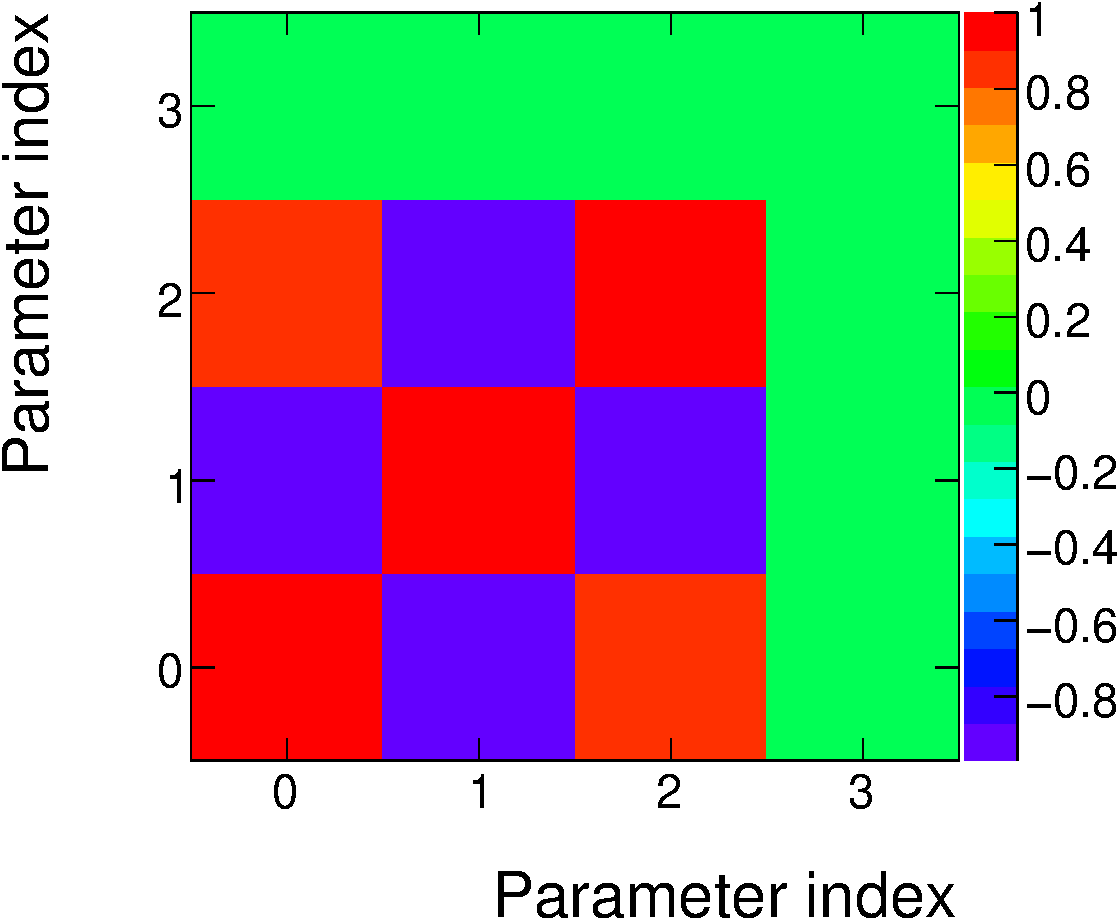
\includegraphics[width=0.45\textwidth]{figures/resFit_ToyMC_PtGenCuts_Correlations}
  \caption{Correlation coefficients of the fitted parameter values
    $\vec{b}$ of the width $\sigma$ of the Gaussian
    resolution. Parameter $3$ corresponds to the slope $\tau$ of the
    spectrum, which is fixed during the fit, and is to be ignored.}
  \label{fig:resFit:toyMC:ptGenCuts:parCorr}
\end{figure}

The fitted parameter values $\vec{b}$ are listed in
Tab.~\ref{tab:resFit:toyMC:ptGenCuts:fitResult}.
They agree with the true values within the statistical uncertainties.

The parameters are strongly (anti-) correlated
(comp. Fig.~\ref{fig:resFit:toyMC:ptGenCuts:parCorr}).
In the present \truth interval, the used
parameterisation of the Gaussian width $\sigma$ is
over-determined.
Hence, omitting either the terms with $b_{0}$ and $b_{2}$ or the term
with $b_{1}$ in~\eqref{eq:resFit:toyMCSigma} would have been
sufficient to describe the measured events.
\textit{Do the fit!!}

\begin{figure}[ht]
  \begin{center}
    \subfigure[]{
      \includegraphics[width=0.45\textwidth]{figures/resFit_ToyMC_PtGenCuts_Sigma}
  } \subfigure[]{
      \includegraphics[width=0.45\textwidth]{figures/resFit_ToyMC_PtGenCuts_SigmaRelDifference}
  }
  \end{center}
  \caption{(a) Relative Gaussian width $\sigma(\pt)/\pt$ evaluated with the fitted
    parameter values (solid line) in comparison to the generated width
    (dashed line).  (b) shows
    the relative difference of the two curves. The shaded area represents the propagated statistical
    uncertainty on the fitted parameter values, taking into account the
    parameter correlations.}
  \label{fig:resFit:toyMC:ptGenCuts:sigma}
\end{figure}

The relative Gaussian width $\sigma(\pt)/\pt$ evaluated with the fitted
parameter values is shown in Fig.~\ref{fig:resFit:toyMC:ptGenCuts:sigma}
in comparison to the true width at generation.
There is good agreement between the fitted and the true resolution
within the statistical uncertainties.
The uncertainties are about $1\%$ at low \pt rising to
about $3\%$ at $\pt \approx 600\gev$ where there is sufficient statistics in
the generated sample (comp. Fig~\ref{fig:resFit:toyMC:ptGenCuts:spectrum}).
For larger \pt the uncertainties rise up to $4.5\%$.

An example of the resulting resolution in comparison to the true
resolution is shown in Fig.~\ref{fig:resFit:toyMC:ptGenCuts:reso} for
one \truth bin.


\subsection{Extension to a data driven event selection}\label{sec:resFit:dataDrivenExt}
So far, events have been selected by cuts on the true jet \pt.
In a more data driven approach the selection is to be applied to the
measured jet \pt.
Events are selected, if for one of the two jets
\begin{equation*}
  \ptmin < \mess < \ptmax.
\end{equation*}
Each event is considered twice; once for a \pt cut on the first and
once for a \pt cut on the second jet.
In this way any bias in the selection arising e.g. from always
selecting the first and thus the jet fluctuated upwards is avoided and the available
statistics is doubled.
As the \pt of the other jet can fluctuate arbitrarily, sensitivity to
the resolution and in particular the non-Gaussian tails is assured
(comp. Fig.~\ref{fig:resFit:ptBinning}).

\begin{figure}[ht]
  \centering
  \includegraphics[width=0.45\textwidth]{figures/PtBinningComp}
  \caption{Comparison of the true resolution in one \pt bin defined by cuts on \ptdijet and on the \pt of a randomly selected jet. In the former, the non-Gaussian tails are surpressed.}
  \label{fig:resFit:ptBinning}
\end{figure}

Cutting on the measured \pt leads to migration effects at the edges of
the selected \pt range due to the finite jet resolution.
Considering the lower limit \ptmin, in an event with \mbox{$\truth <
  \ptmin$} the actually measured jet \pt might fluctuate upwards
resulting in \mbox{$\mess > \ptmin$} and thus false acceptance of the
event.
Similarly, events might be falsely rejected due to downward fluctuations.
Since the dijet cross section is steeply falling with \pt, the
described migration is asymmetric i.e. there is more upward
than downward migration and more events are falsely accepted.
(Analogue considerations hold true for the upper limit.)
The described migration effects are demonstrated in
Fig.~\ref{fig:resFit:toyMC:ptCuts:spectrum}.

\begin{figure}[ht]
  \begin{center}
    \subfigure[]{
      \includegraphics[width=0.45\textwidth]{figures/resFit_ToyMC_PtCuts_SpectrumLog}
    } \subfigure[]{
      \includegraphics[width=0.45\textwidth]{figures/resFit_ToyMC_PtCuts_SpectrumLinear}
    }
  \end{center}
  \caption{Simple simulation of a sample of ideal dijet
    events. Generated \truth spectrum (histogram) and the underlying pdf (solid
    line) after cuts on measured \pt. The spectrum is shown (a) in log
    scale and (b) in linear scale.}
  \label{fig:resFit:toyMC:ptCuts:spectrum}
\end{figure}

\begin{figure}[ht]
  \begin{center}
    \subfigure[]{
      \includegraphics[width=0.45\textwidth]{figures/resFit_ToyMC_PtCuts_ResolutionBin1}
   } \subfigure[]{
      \includegraphics[width=0.45\textwidth]{figures/resFit_ToyMC_PtCuts_ResolutionBin7}
   }
  \end{center}
  \caption{Simple simulation of a sample of ideal dijet
    events. Generated true resolution \mbox{$\mess / \truth$} (histogram) and the fitted
    resolution (solid line) in two different \truth bins after cuts on measured \pt.}
  \label{fig:resFit:toyMC:ptCuts:reso}
\end{figure}

\begin{figure}[ht]
  \begin{center}
    \subfigure[]{
      \includegraphics[width=0.45\textwidth]{figures/resFit_ToyMC_PtCuts_Sigma}
  } \subfigure[]{
      \includegraphics[width=0.45\textwidth]{figures/resFit_ToyMC_PtCuts_SigmaRelDifference}
  }
  \end{center}
  \caption{(a) Relative Gaussian width $\sigma(\pt)/\pt$ evaluated with the fitted
    parameter values (solid line) in comparison to the generated width
    (dashed line). The fit has been performed after cuts on measured \pt. (b) shows
    the relative difference of the two curves. The shaded area represents the propagated statistical
    uncertainty on the fitted parameter values, taking into account the
    parameter correlations.}
  \label{fig:resFit:toyMC:ptCuts:sigma}
\end{figure}

The dijet pdf~\eqref{eq:resFit:dijetPdf} is adapted to include the
cuts on the measured jet \pt.
First, the allowed range of measured \pt is restricted for the
jet the \pt cut is applied to.
W.l.o.g. it is assumed that this is the first jet; the pdfs of
measured jet \pt therefore become
\begin{eqnarray*}
  f_{\vec{b}}\left(\meas{1}|\truth\right) & = & 
  \frac{1}{\mathcal{N}_{1}}\exp\left[-\frac{1}{2}\left(\frac{\meas{1}
        - \truth}{\sigma}\right)^{2}\right]
  \cdot\theta\left(\meas{1} - \ptmin\right)
  \cdot\theta\left(\ptmax - \meas{1}\right) \\
  f_{\vec{b}}\left(\meas{2}|\truth\right) & = & 
  \frac{1}{\mathcal{N}_{2}}\exp\left[-\frac{1}{2}\left(\frac{\meas{2}
        - \truth}{\sigma}\right)^{2}\right] \\
\end{eqnarray*}
with the normalisation constants
\begin{eqnarray*}
  \mathcal{N}_{1} & = &
  \int^{\ptmax}_{\ptmin}\dif{\meas{1}}\,f_{\vec{b}}\left(\meas{1}|\truth\right)
  = \sqrt{\frac{\pi}{2}}\sigma \left[ \text{erf}\left(\frac{\ptmax -
        \truth}{\sqrt{2}\sigma}\right) - \text{erf}\left(\frac{\ptmin
        - \truth}{\sqrt{2}\sigma}\right)\right] \\
  \mathcal{N}_{2} & = &
  \int^{\infty}_{0}\dif{\meas{2}}\,f_{\vec{b}}\left(\meas{2}|\truth\right)
  = \sqrt{\frac{\pi}{2}}\sigma \left[ 1 +
    \text{erf}\left(\frac{\truth}{\sqrt{2}\sigma}\right)\right]
  \approx \sqrt{2\pi}\sigma.
\end{eqnarray*}
Second, the pdf of the true \pt is extended to incorporate the events
migrating into the allowed \pt range by
\begin{equation}
  \label{eq:resFit:toyMC:ptCuts:extendedSpectrum}
  \tilde{f}\left(\truth\right) = \frac{1}{\mathcal{N}_{\tilde{f}}}
  f\left(\truth\right) \int^{\ptmax}_{\ptmin}\dif{x}\,f_{\text{MC}}\left(x|\truth\right)
\end{equation}
with the normalisation
\begin{equation*}
  \mathcal{N}_{\tilde{f}} = \int^{\infty}_{0}\dif{\truth}\,
  f\left(\truth\right) \int^{\ptmax}_{\ptmin}\dif{x}\,f_{\text{MC}}\left(x|\truth\right).
\end{equation*}
Here, $f(\truth)$ denotes the underlying spectrum~\eqref{eq:resFit:toyMCSpec} and
$f_{\text{MC}}(x|\truth)$ the pdf of measured \pt.
$f_{\text{MC}}(x|\truth)$ in \eqref{eq:resFit:toyMC:ptCuts:extendedSpectrum} is taken from the
simulation and the parameters are kept fixed during the maximisation.
Thus usage of the simulation introduces a further uncertainty but they
are small as in case of the underlying spectrum as shown below.
The adapted dijet pdf then becomes
\begin{equation}
  \label{eq:resFit:toyMC:ptCuts:pdf}
  f_{\vec{b}}\left(\meas{1},\meas{2}\right) = \int^{\infty}_{0}\dif{\truth}\,\tilde{f}\left(\truth\right)
  \cdot f_{\vec{b}}\left(\meas{1}|\truth\right)
  \cdot f_{\vec{b}}\left(\meas{2}|\truth\right),
\end{equation}
which is properly normalised to
\begin{equation*}
  1 = \int^{\ptmax}_{\ptmin}\dif{\meas{1}}\,\int^{\infty}_{0}\dif{\meas{2}}\, f_{\vec{b}}\left(\meas{1},\meas{2}\right).
\end{equation*}

\begin{table}[ht]
  \centering
  \begin{tabular}[ht]{lccc}
    \hline \hline
    $b_{i}$ & $0$ & $1$ & $2$ \\
    \hline
    True value & $4$           & $1.2$                   & $0.05$ \\
    Fit result   & $4 \pm 1$ & $1.20 \pm 0.07$ & $0.049 \pm 0.005$ \\
    \hline \hline
  \end{tabular}
  \caption{Parameter values of the width $\sigma(\pt)$ of the Gaussian
    resolution. Listed are the true values used for the generation and
    the fitted values. The fit has been performed after cuts on measured \pt.
    The uncertainties assigned to the fitted values
    are the statistical uncertainties from the fit; correlations are not shown.}
  \label{tab:resFit:toyMC:ptCuts:fitResult}
\end{table}

Again the sample of ideal dijet events is used to test the discussed extension of the method.
Cuts are placed on the measured \pt at \mbox{$\ptmin = 80\gev$} and \mbox{$\ptmax = 800\gev$} (comp. Fig.~\ref{fig:resFit:toyMC:ptCuts:spectrum}).
The jet energy resolution of the selected dijet events is fitted using the modified pdf~\eqref{eq:resFit:toyMC:ptCuts:pdf}.
Uncertainties due to uncertainties in the description of the spectrum are discussed in Section~\ref{sec:resFit:toyMC:uncert}.

The fitted parameter values $\vec{b}$ of the Gaussian width $\sigma$ are listed in
Tab.~\ref{tab:resFit:toyMC:ptCuts:fitResult}.
They agree with the true values within the statistical uncertainties.
As expected, they feature the same correlation pattern as in case of \ptgen cuts.

The relative Gaussian width $\sigma(\pt)/\pt$ evaluated with the fitted
parameter values is shown in Fig.~\ref{fig:resFit:toyMC:ptCuts:sigma}
in comparison to the true width at generation.
There is good agreement between the fitted and the true resolution
within the statistical uncertainties.
As before, the uncertainties are about $1\%$ at low \pt rising to
about $3\%$ at $\pt \approx 600\gev$ and up to $4.5\%$ at very large
\pt.
An example of the resulting resolution in comparison to the true
resolution is shown in Fig.~\ref{fig:resFit:toyMC:ptCuts:reso} for
one \truth bin.

It can be concluded therefore that the method is working also for a data driven event selection.



\subsection{Estimation of systematic uncertainties}\label{sec:resFit:toyMC:uncert}

The dijet pdf discussed above contains knowledge of the actual dijet spectrum and --- in case of cuts on measured jet \pt --- also of the resolution to describe the cut-off effects.
When applying the method to data this information would be taken from a MC simulation.
Test have been performed to evaluate the influence of uncertainties in the MC description on the fitted resolution.

\begin{figure}[ht]
  \centering
  \includegraphics[width=0.45\textwidth]{figures/resFit_ToyMC_PtCuts_SigmaUncertainties}
  \caption{Relative differences of the Gaussian widths $\sigma(\pt)$ evaluated with the fitted
    parameter values for different variations of the spectrum and the correct spectrum.}
  \label{fig:resFit:toyMC:uncert:systUncertainties}
\end{figure}

\begin{table}[ht]
  \centering
  \begin{tabular}[ht]{lccc}
    \hline \hline
    $b_{i}$ & $0$ & $1$ & $2$ \\
    \hline
   Correct            & $4 \pm 1$ & $1.20 \pm 0.07$ & $0.049 \pm 0.005$ \\
   Spectrum $+30\%$   & $3 \pm 2$ & $1.22 \pm 0.07$ & $0.049 \pm 0.005$ \\
   Spectrum $-30\%$   & $5 \pm 1$ & $1.19 \pm 0.08$ & $0.052 \pm 0.006$ \\
   Resolution $+30\%$ & $5 \pm 1$ & $1.13 \pm 0.07$ & $0.054 \pm 0.004$ \\
   Resolution $-30\%$ & $5 \pm 2$ & $1.19 \pm 0.08$ & $0.050 \pm 0.006$ \\
    \hline \hline
  \end{tabular}
  \caption{Parameter values of the width $\sigma(\pt)$ of the Gaussian
    resolution. Listed are the true values used for the generation and
    the fitted values. The uncertainties assigned to the fitted values
    are the statistical uncertainties from the fit.}
  \label{tab:resFit:toyMC:uncert:fitResult}
\end{table}

The fit has been repeated with the same setup as described in Section~\ref{sec:resFit:dataDrivenExt}.
In order to evaluate the influence of the spectrum on the result the slope i.e. the parameter $\tau$ in \eqref{eq:resFit:toyMCSpec} has been varied by $\pm30\%$.
Cut-off effects in the spectrum are described by the true resolution $f_{\text{MC}}(x|\truth)$ in \eqref{eq:resFit:toyMC:ptCuts:extendedSpectrum}.
All three parameters $b_{\text{MC},i}$ of $f_{\text{MC}}(x|\truth)$ have been varied by $\pm30\%$ to evaluate uncertainties arising from the simulation.

The fitted parameter values for each variation are listed in Tab.~\ref{tab:resFit:toyMC:uncert:fitResult} in comparion to the values obtained when using the correct spectrum.
The relative differences of the Gaussian widths $\sigma$ calculated with these fitted parameter values to the $\sigma$ using the correct spectrum are presented in Fig.~\ref{fig:resFit:toyMC:uncert:systUncertainties} as a function of \pt for the different variations; they are below $4\%$.
A varied spectrum predominantly results in a larger resolution.



\subsection{Application to a realistic QCD simulation}\label{sec:resFit:qcdSelection}
The method has then been applied to QCD events with 7\tev center of
mass energy which were generated with PYTHIA and went through a full
GEANT4 based CMS detector simulation\footnote{The used dataset is
  \texttt{/QCDFlat\_Pt15to3000/Summer09-MC\_31X\_V9\_7TeV-v1/GEN-SIM-RECO}}.
Jets have been reconstructed from calorimeter towers using the
anti-$k_{T}$ algorithm with size parameter $R=0.5$.
The jet energy scale has been corrected for $\eta$ and \pt dependence
by the appropriate L2L3 corrections\footnote{These are the
  \texttt{JetMETCorrections.Configuration.L2L3Corrections\_Summer09\_7TeV\_ReReco332\_cff}
corrections.}.

\begin{figure}[ht]
  \begin{center}
    \subfigure[]{
      \label{fig:resFit:qcd:dijetspectrum:subA}
      \includegraphics[width=0.45\textwidth]{figures/resFit_QCD_MCSpectrum}
    } \subfigure[]{
      \label{fig:resFit:qcd:dijetspectrum:subB}
      \includegraphics[width=0.45\textwidth]{figures/resFit_QCD_MCTruthResolution}
    }
  \end{center}
  \caption{(a) \ptgen distribution and (b) MC truth resolution of the leading two jets in the selected dijet sample.
    The solid lines are fits of the indicated functions.}
  \label{fig:resFit:qcd:dijetspectrum}
\end{figure}

In the following jets are considered to be ordered in corrected
measured jet \pt.
Dijet events are selected by requiring the third jet to have small \pt
compared to the leading two jets,
\begin{enumerate}
\item $\ptrel < 0.1$ with $\ptrel = \frac{2\ptsub{3}}{\ptsub{1} + \ptsub{2}}$.
\end{enumerate}
This selection cut has been adopted from~\cite{CMSAN-2008/031}.
The additional cut on $\Delta\phi$ performed there has been dropped as it has been found to be strongly correlated to the cut on \ptrel.
In order to reject jets clustered from calorimeter noise a cut on the
electromagnetic fration of the two leading jets is applied,
\begin{enumerate}
\item[2.] $0.01 < f_{\text{em},i} < 0.99$ with $i\in\{1,2\}$.
\end{enumerate}

So far and in the following, the resolution is defined as a function
of jet \pt.
It is influenced for example by the magnetic solenoid field which
 bends charged particles out of the jet cone depending on their \pt.
Other effects such as the intrinsic calorimeter resolution are energy $E$
dependent.
The dependence on the difference between the $E$ and \pt is minimised by
considering dijet events with both leading jets in a restricted $\eta$ region,
\begin{enumerate}
\item[3.] $|\eta_{i}| < 1.2$ with $i\in\{1,2\}$.
\end{enumerate}
It is planned to apply the method to different $\eta$ regions taking
into account also those events in which the two leading jets are in
different $\eta$ regions.

The events are weighted corresponding to an integrated
luminosity of $100\,\text{pb}^{-1}$.

The resulting \ptgen spectrum is shown in Fig.~\ref{fig:resFit:qcd:dijetspectrum:subA}.
It is fitted with an empiric function
\begin{equation}
  \label{eq:resFit:qcd:ptGenSpectrum}
  f\left(\ptgen\right) = \sum^{2}_{i=0}\,\exp\left[-\left(a_{2i} + a_{2i+1}\ptgen\right)\right]
\end{equation}
to have a first applicable parameterisation of the spectrum
$f(\truth)$.
The fitted parameter values $a_{i}$ are listed in
Table~\ref{tab:resFit:qcd:dijetspectrum} and the resulting pdf is
superimposed in Fig.~\ref{fig:resFit:qcd:dijetspectrum:subA}.
\begin{table}[ht]
  \centering
  \begin{tabular}{rc}
    \hline
    \hline
    $a_{i}$ & Fitted value \\
    \hline
    $0$ & $0.56 \pm 0.04$ \\
    $1$ & $0.0300 \pm 0.0004$ \\
    $2$ & $3.91 \pm 0.09$ \\
    $3$ & $0.0152 \pm 0.0004$ \\
    $4$ & $7.15 \pm 0.05$ \\
    $5$ & $0.00837 \pm 0.00008$ \\
    \hline
    \hline
  \end{tabular}
 \caption{Fitted parameter values of the dijet \ptgen spectrum.}
  \label{tab:resFit:qcd:dijetspectrum}
\end{table}

\begin{figure}[ht]
  \centering
  \includegraphics[width=0.45\textwidth]{figures/resFit_PtDependentSigma}
  \caption{Width $\sigma$ of a Gaussian resolution in QCD dijet events. Shown is $\sigma$ from fitted parameter values (red line) in comparison to the truth from the MC simulation (blue line).}
  \label{fig:resFit:qcd:ptDependentSigma}
\end{figure}

The determination of a Gaussian resolution~\eqref{eq:resFit:toyMCRes}
with a \pt dependent width $\sigma$ as in~\eqref{eq:resFit:toyMCSigma}
has been performed as for the ideal sample above.
The results are not satisfying (comp. Fig.~\ref{fig:resFit:qcd:ptDependentSigma}).

Various test have been performed and the method appears to work fine
for a moderately falling \pt spectrum.
In case of a realistic QCD spectrum
(comp. Fig.~\ref{fig:resFit:qcd:dijetspectrum:subA}), however, the
determined resolution does not describe the true resolution at large
\pt anymore.
The failure of the method is assumed to be due to the non-ideal
topology of the selected dijet events, namely the presence of a third
jet.
Presumeably compensation of the non-dijet configurations at low \pt,
where by far the most events are situated, has more influence on the
fit result than accurate description of the resolution of the few high
\pt events.
These effects and an extension of the presented method are under
study.
Meanwhile a modified strategy to determine the resolution is
investigated and presented in the following sections.


\section{Determination of the mean Gaussian resolution in \pt bins}
\subsection{Strategy}
The mean Gaussian resolution with constant width $\bar{\sigma}$ is to be determined in bins of \pt.
Afterwards it is interpolated between the bins with a continuous function.
The bin size is chosen as a compromise between having small bins for a
differential measurement and sufficient statistics in each bin.

Dijet events are selected by the cuts described in Section~\ref{sec:resFit:qcdSelection} from the same QCD sample.
Bins are defined by cuts on the measured jet \pt as described in Section~\ref{sec:resFit:dataDrivenExt}.
Table~\ref{tab:resFit:qcd:ptBins} lists the chosen binning.

\begin{table}[ht]
  \centering
  \begin{tabular}{rcc}
    \hline
    \hline
    Bin & \ptmin (\gev) & \ptmax (\gev) \\
    \hline
    0 & 100 & 120 \\
    1 & 120 & 140 \\
    2 & 140 & 170 \\
    3 & 170 & 200 \\
    4 & 200 & 250 \\
    5 & 250 & 300 \\
    6 & 300 & 400 \\
    7 & 400 & 600 \\
    8 & 600 & 1000 \\
    \hline
    \hline
  \end{tabular}
  \caption{Definition of \pt bins for the fit of the mean Gaussian resolution.}
  \label{tab:resFit:qcd:ptBins}
\end{table}

The modified spectrum $\tilde{f}(\truth)$ from~\eqref{eq:resFit:toyMC:ptCuts:extendedSpectrum} is utilised in the fit.
The underlying spectrum $f(\truth)$ is described by~\eqref{eq:resFit:qcd:ptGenSpectrum} with the parameter values listed in Tab.~\ref{tab:resFit:qcd:dijetspectrum}.
Cut-off effects are included as before using the true -- and \pt dependent -- resolution $f_{\text{MC}}(x|\truth)$ in $\tilde{f}(\truth)$.
$f_{\text{MC}}(x|\truth)$ has been determined by fitting the $\pt/\ptgen$ distributions in small $\ptgen$ bins with a central Gaussian.
The widths of the Gaussians are shown in Fig.~\ref{fig:resFit:qcd:dijetspectrum:subB}.
They are fitted with the continous function
\begin{equation}
  \label{eq:resFit:qcd:sigma}
  \frac{\sigma}{\pt} = \frac{b_{1}\sqrt{\gev}}{\sqrt{\pt}} \oplus \frac{b_{2}\gev}{\pt}.
\end{equation}
(In this \pt range there is no sensitivity to a third term $b_{0}$, which is why it is omitted.)
The values $b_{i}$ of the true resolution\footnote{The fit is applied once to the presented Fig.~\ref{fig:resFit:qcd:dijetspectrum:subB} and once to an analogue plot with a logarithmic binning in \ptgen.
The parameters listed in Tab.~\ref{tab:resFit:qcd:resolution} are the mean values from the two fits.}
are listed in Tab.~\ref{tab:resFit:qcd:resolution}.

Figure~\ref{fig:resFit:qcd:specExBin} shows the \ptgen spectrum in an example bin.
It is well described by $\tilde{f}(\truth)$.


\subsection{Results for a QCD simulation}
\begin{figure}[ht]
  \begin{center}
    \subfigure[]{
      \label{fig:resFit:qcd:specExBin}
      \includegraphics[width=0.45\textwidth]{figures/resFit_QCD_Gauss_Spectrum_PtBin3}
    } \subfigure[]{
      \label{fig:resFit:qcd:extrapolationExBin}
      \includegraphics[width=0.45\textwidth]{figures/resFit_QCD_Gauss_ExtrapolatedSigma_PtBin3}
    }
  \end{center}
  \caption{(a) \ptgen distribution and of the leading two jets in an example \pt bin.
    The solid line is the spectrum $\tilde{f}(\truth)$.
    (b) Fitted Gaussian mean widths $\bar{\sigma}/\pt$ for different cuts on \ptrel in the same example \pt bin.
    The solid line is a linear fit to extrapolate $\bar{\sigma}/\pt$ for ideal dijet events.}
\end{figure}

The fit has been performed for the listed \pt bins.
The result is affected by the presence of a third jet.
For example, the mean resolution for jets with \mbox{$170 < \pt < 200\gev$} has been determined to \mbox{$\bar{\sigma}/\bar{\pt} = 0.136 \pm 0.002$} whereas the MC truth value is \mbox{$0.0933$}.
This difference is dependent on the maximum \ptrel as demonstrated in Fig.~\ref{fig:resFit:qcd:extrapolationExBin}, which shows the fitted mean resolution for different values of \ptrel.
There is a linear trend visible.
In order to extrapolate to the results to the case of an ideal dijet event, the $\bar{\sigma}\/\pt$ are fitted with a linear function and the y axis intercept is considered as the correct jet energy resolution.

The extrapolated Gaussian mean widths $\bar{\sigma}/\pt$ found in this way are shown for different \pt bins in Fig.~\ref{fig:resFit:qcd:extrapolation}.
Here, the \pt values are the mean values of the assumed spectra $\tilde{f}(\truth)$ in each bin.
The shown statistical uncertainties are combined from two sources.
\begin{enumerate}
\item The first contribution is the statistical uncertainty on the
  parameter of y axis intercept in the linear extrapolation (comp.
  Fig.~\ref{fig:resFit:qcd:extrapolationExBin}).
\item The second contribution arises from the uncertainty due to the statistics in
  the used MC sample.
  As the event weights are large for small \pt, statistical fluctations might become significant.
  To evaluate this uncertainty, the same fits have been performed again without event weights (for the used sample this corresponds to a flattened QCD spectrum).
  The statistical uncertainties obtained in this case on the y axis intercept are added in quadrature to the ones in 1.
\end{enumerate}

The dashed line in Fig.~\ref{fig:resFit:qcd:extrapolation} represents the MC truth resolution.
The fitted values are in reasonable agreement with the MC truth.
They are then fitted with the continous function \eqref{eq:resFit:qcd:sigma} (solid line).
The parmeters of this fit are listed in Tab.~\ref{tab:resFit:qcd:resolution}.

\begin{table}[ht]
  \centering
  \begin{tabular}[ht]{lcc}
    \hline \hline
    $b_{i}$ & $1$ & $2$ \\
    \hline
    MC truth    & $1.145 \pm 0.001$ & $0.0370 \pm 0.0006$ \\
    Fit result  & $1.18  \pm 0.04$  & $0.032  \pm 0.007$ \\
    \hline \hline
  \end{tabular}
  \caption{Parameter values of the width $\sigma(\pt)$ of the Gaussian resolution~\eqref{eq:resFit:qcd:sigma}.
    Listed are the MC truth values and the fitted values.
    For the fit, the mean $\bar{\sigma}/\pt$ has been fitted in different \pt bins and the result fitted again with the continous function~\eqref{eq:resFit:qcd:sigma} (comp. Fig.~\ref{fig:resFit:qcd:extrapolation}).
    The uncertainties assigned to the fitted values are the statistical uncertainties.}
  \label{tab:resFit:qcd:resolution}
\end{table}

\begin{figure}[ht]
  \begin{center}
    \subfigure[]{
      \label{fig:resFit:qcd:extrapolation}
      \includegraphics[width=0.45\textwidth]{figures/resFit_QCD_Gauss_ExtrapolatedResolution}
    } \subfigure[]{
      \label{fig:resFit:qcd:systUncert}
      \includegraphics[width=0.45\textwidth]{figures/resFit_QCD_Gauss_SystematicUncertainties}
    }
  \end{center}
  \caption{(a) Gaussian mean widths $\bar{\sigma}/\pt$ from extrapolation \mbox{$\ptrel\rightarrow0$} in different \pt bins.
  The \pt values are the mean values of the assumed spectra $\tilde{f}(\truth)$ in each bin.
  The error bars indicate the combined statistical uncertainties from the extrapolation and the MC statistics.
  The solid line is a fit to the $\bar{\sigma}/\pt$, the dashed line shows the MC truth resolution for comparison.
  (b) Estimation of systematic uncertainties.
  The lines represent relative differences of the resolution for different variations of the spectrum to the correct spectrum.}
\end{figure}
\clearpage

\subsection{MHT spectrum}
In order to evaluate the influence of non-Gaussian tails in the resolution to the MHT spectrum, a simple generator level based jet smearing has been performed.
The same dijet selection as presented in Sec.~\ref{sec:resFit:qcdSelection} has been applied.
For this demonstration, the \ptgen of the leading two jets has been weighted with a random number from a Gaussian resolution pdf, where $\sigma$ has been parameterised using the MC truth values listed in Tab.~\ref{tab:resFit:qcd:resolution}.

\begin{figure}[ht]
  \begin{center}
    \subfigure[]{
      \includegraphics[width=0.45\textwidth]{figures/MHTSpectrumGauss}
    } \subfigure[]{
      \includegraphics[width=0.45\textwidth]{figures/MHTRatioGauss}
    }
  \end{center}
  \caption{(a) MHT from the two leading jets in a QCD dijet sample (marker) and prediction from smearing of the corresponding generator level jets with the true Gaussian resolution (line).
    (b) Ratio of prediction and truth.}
\label{fig:resFit:qcd:mhtGauss}
\end{figure}

In Fig.~\ref{fig:resFit:qcd:mhtGauss} the MHT spectrum resulting from the weighted \ptgen of the two jets is compared to the MHT spectrum from the corresponding measured jet \pt.
The actual MHT is underestimated by about $5\%$ up to 200\gev.
Above, which are $\approx2\%$ of all the events, the MHT is underestimated by $\approx50\%$.
This difference is explained by the presence of non-Gaussian tails in the resolution which were not considered.



\section{Determination of a non-Gaussian resolution}



% If $f$ and $r$ are parameterised in a suitable form using the
% parameters $\mathbf{b}$, the probability $\mathcal{P}^{1,2}_{i}$
% becomes a function of $\mathbf{b}$.  For a sample of
% $N_{\mathrm{dijet}}$ dijet events it is therefore possible to define
% the likelihood
% \begin{equation}
%   \label{eq:respFit_Likelihood}
%   \mathcal{L}(\mathbf{b}) = \prod^{N_{\mathrm{dijet}}}_{i=0} \mathcal{P}^{1,2}_{i}(\mathbf{b}) 
% \end{equation}
% which has to be maximised to find the optimal values of the parameters
% $\mathbf{b}$.  For technical reasons, the negative logarithm of
% $\mathcal{L}$ is minimised.

% It is worth to note that an appropriate definition of the probability
% density $\mathcal{P}$ of the event configuration allows to include
% other data types into the likelihood in \eqref{eq:respFit_Likelihood}
% e.g. 3-jet or photon+jet events.


% \paragraph{Parameterisation}
% The central part of the jet response function has a Gaussian shape.
% For an accurate estimation of the \met spectrum however, also the
% non-Gaussian tail of the response should be described.  Although parts
% of the tail are due to known physical effects such as jets containing
% heavy flavour quarks, an empirical approach is chosen for its
% description to be able to include any unknown effects.  Therefore, the
% response pdf is parameterised as a superposition of a Gaussian and an
% interpolated step function
% \begin{equation*}
%   r(R,\pttrue;\mathbf{b}) = c \cdot G(R;\mu_{0},\sigma(\pttrue)) + (1-c) \cdot S_{N}(R;\mathbf{b}).
% \end{equation*}
% Here, $G$ is a Gaussian describing the central bulk part of the
% response and $S_{N}$ an interpolated step function describing the
% non-Gaussian tail of the response.  This is illustrated in
% Fig.~\ref{fig:respFit_ResponsePDF}.
% \begin{figure}[ht]
%   \begin{center}
%     \includegraphics[width=\textwidth]{./RespFit_RespPDFSketch}
%   \end{center}
%   \caption{Sketch of the response parameterisation.}
%   \label{fig:respFit_ResponsePDF}
% \end{figure}

% The Gaussian $G$ is normalised to unity.  The width $\sigma$ is
% $\pttrue$ dependent by
% \begin{equation*}
%   \sigma(\pttrue) = \frac{a_{1}}{\pttrue} \oplus \frac{a_{2}}{\sqrt{\pttrue}} \oplus a_{3},
% \end{equation*}
% where the parameters $a_{i}$ are determined by the fit
% i.e.~\mbox{$a_{i}\in\mathbf{b}$}.  The center $\mu_{0}$ of the
% Gaussian corresponds to the jet energy scale and has to be fixed
% during the fit.  Otherwise any assymmetric parts of the response
% distribution would be absorbed in the Gaussian by shifting the scale
% $\mu_{0}$, thus preventing a handle on the non-Gaussian tails.  If
% corrected jets are chosen for the analysis, $\mu_{0}$ is ideally one.

% $S_{N}$ is a step function with $N$ steps, and the function values
% $S_{N}(R_{i})$ of each step corresponds to one free parameter.  It is
% normalised to unity, too.  This normalisation introduces an additional
% degree of freedom.  It is absorbed by fitting only $N-1$ parameters
% and constraining the $N$th parameter by the normalisaton requirement
% e.g.~\mbox{$S_{N}(R_{i})\in\mathbf{b}$}
% for~\mbox{$i\in\left\{1,2,\ldots N-1\right\}$}.  In order to improve
% the behaviour of the fit, continuity of the step function is ensured
% by linear interpolation between the function values of adjacent steps.
% Thus
% \begin{equation*}
%   S_{N}(R) = \Delta R \cdot S_{N}(R_{i}) + (1-\Delta R) \cdot S_{N}(R_{i+1}),
% \end{equation*}
% where $R_{i}$ is the response at the center of one step and $\Delta R$
% is the distance~\mbox{$R - R_{i}$}.

% The relative contributions of $G$ and $S$ to $r$ is controlled by the
% normalisation constant $c$ which is another fitted parameter
% i.e.~\mbox{$c\in\mathbf{b}$}.

% The possible values of $c$ as well as the step function values
% $S_{N}(R_{i})$ are limited: \mbox{$0 \leq c \leq 1$} and \mbox{$0 \leq
%   S_{N}(R_{i})$}.  In the fit, this is ensured by appropriate penalty
% terms in the likelihood which diverge quadratically as one of the
% parameters crosses its limits.

% In contrast to the Gaussian part, there is no \pttrue dependence of
% the step function.  The chosen strategy is to perform independent fits
% in different bins of \pt, resulting in a set of response pdfs, one for
% each bin in \pt.  Likewise, different response pdfs are fitted for
% different $\eta$ bins.

% \begin{figure}[ht]
%   \begin{center}
%     \includegraphics[width=0.5\textwidth]{RespFit_PtGenSpectrumWOCuts}
%   \end{center}
%   \caption{Demonstration of migration due to cuts on \ptdijet.}
%   \label{fig:respFit_ExMigration}
% \end{figure}

% In principle the binning has to be done in true \pt and $\eta$.
% However, bins are to be defined in measurable quantities.  Therefore
% \begin{equation*}
%   \ptdijet = \frac{1}{2}\left(\pt^{1} + \pt^{2}\right)
% \end{equation*}
% the mean measured jet \pt in the dijet event is chosen as binning
% variable in \pt.

% The binning in measured \ptdijet leads to migration effects
% w.r.t. \pttrue due to the width of the jet response.  Considering a
% lower cut on \ptdijet, in an event with \pttrue lower than that cut
% value, the actually measured jet \pt might fluctuate upwards leading
% to \ptdijet larger than the cut value and thus false acceptance of the
% event.  Similarly, events might be falsely rejected due to downward
% fluctuations.  Since the dijet cross section is steeply falling with
% \pt, the described migration is asymmetric i.e. there is more upward
% than downward migration and more events are falsely accepted.  These
% migration effects are demonstrated in
% Fig.~\ref{fig:respFit_ExMigration}.

% In contrast, the dijet cross section is more flat in $\eta$ and the
% $\eta$ resolution of the calorimeter is with \mbox{$\sigma/\eta = ??$}
% small in comparison.  Migration effects due to the binning in measured
% $\eta$ are therefore neglected.

% \begin{figure}[ht]
%   \begin{center}
%     \includegraphics[width=0.5\textwidth]{RespFit_TruthPDFToyMCEx}
%   \end{center}
%   \caption{Description of the migration due to cuts on \ptdijet.}
%   \label{fig:respFit_TruthPDFToyMCEx}
% \end{figure}

% The description of the migration effects due to the cuts on \ptdijet
% can be included into the parameterisation of the truth pdf $f$ by
% \begin{equation}
%   \label{eq:respFit_TruthPDF}
%   f(\pttrue,\mathbf{b}) \propto \hat{f}(\pttrue,\mathbf{b})\int^{p^{\mathrm{dijet}}_{\mathrm{T,max}}}_{p^{\mathrm{dijet}}_{\mathrm{T,min}}} \mathrm{d}x\,\frac{r(x/\pttrue,\mathbf{b})\pttrue}{\sqrt{2}}.
% \end{equation}
% Here, $\hat{f}(\pttrue,\mathbf{b})$ denotes the truth pdf in the pure
% case without any cuts.  For the time being it is assumed to follow a
% powerlaw and to fall with~$\propto1/(\pttrue)^{n}$, where $n$ is a
% parameter determined by the fit i.e.~\mbox{$n\in\mathbf{b}$}.  The
% integral then describes the migration effects;
% $p^{\mathrm{dijet}}_{\mathrm{T,min}}$ and
% $p^{\mathrm{dijet}}_{\mathrm{T,max}}$ are the lower and the upper cut
% on \ptdijet, respectively, and $r$ is again the jet response pdf.

% This can be demonstrated using a simple dijet (Toy Monte Carlo)
% simulation.  The true \pt is generated according to a pdf
% falling~$\propto1/(\pttrue)^{7}$ for~\mbox{$100 < \pttrue <
%   600\,\gev$}.  For each event, two measured \pt are generated from a
% Gaussian pdf of width~$1/\sqrt{\pttrue}$ and mean value on.  Events
% are selected if~\mbox{$200 < \ptdijet < 400\,\gev$}.  The resulting
% \pttrue spectrum is shown in Fig.~\ref{fig:respFit_TruthPDFToyMCEx}.
% It is well described by \eqref{eq:respFit_TruthPDF} if the correct
% pure spectrum~\mbox{$\hat{f}\propto1/(\pttrue)^{7}$} and
% response~\mbox{$r\propto1/\sqrt{\pttrue}$} are used.


% \paragraph{Event selection}

% % This should go somewhere to the event selection, mentioning
% % what effects are included in the measured resolution
% The partons in an event undergo a fragmentation and hadronisation
% process to form particle jets.  The transverse momentum \pt of these
% jets is mismeasured in the calorimeter due to various effects like for
% example particles that are invisible to the calorimeter
% (e.g. neutrinos) or the intrinsic calorimeter response.  This process
% is modeled by the convolution of the probability density functions,
% \textit{pdf}s, of the \pt spectrum of the jets and of the detector
% response.


% The presented studies are performed on the Summer08 QCD samples
% generated with \PYTHIA.  Jets are reconstructed using the SisCone5 jet
% algorithm and the Summer08 MC L2 and L3 jet energy corrections are
% applied.  The events are weighted for a luminosity of $100\,pb^{-1}$.

% The response fit method assumes only two jets in an event.  In that
% case the \pt balance is only affected by the calorimeter response --
% which is to be measured -- while effects such as hard gluon radiation
% are not present.  In order to select events fullfilling these
% conditions, dijet selection cuts similar to those used for the
% determination of the relative jet energy correction (\texttt{CMS
%   AN-2008/031}) are applied:
% \begin{itemize}
% \item 2 jets leading in \pt with $|\eta| < 0.8$,
% \item $\pt^{3} / \pt^{\mathrm{dijet}} < 0.1$ or $\pt^{3} < 2\,\gev$,
%   where $\pt^{\mathrm{dijet}} = (\pt^{1} + \pt^{2})/2$,
% \item $|\Delta\phi^{1,2}| > 2.7$.
% \end{itemize}
% Additionally, the hadronic fraction of both the leading jets is
% limited to \mbox{$0.07 < \pt^{\mathrm{had}} / \pt^{\mathrm{jet}} <
%   0.95$}.  Note that the above cuts are performed after the jet energy
% corrections are applied.

% The validation plots presented in the following compare the fitted
% response with the true response $\pt / \ptgen$ in the simulation,
% where \ptgen denotes the \pt of the jet on generator level.  It is
% therefore crucial that the correct generator level jet is assigned to
% a calorimeter level jet.  In order to ensure this, the distance
% $\Delta R$ in $(\eta,\phi)$ space between the jet and the generator
% jet is required to be
% \begin{equation*}
%   \Delta R(\mathtt{genjet},\mathtt{jet}) < 0.1.
% \end{equation*}
% Of course, this cut cannot be performed on data and is done here
% sorely for validatiion purposes.  It has been checked that the fit
% returns the same results with or without applying the $\Delta R$ cut.


% \paragraph{Conceptual study for one bin}
% \begin{itemize}
% \item \textit{Details of the fit: iterations, fixed cut integral}
% \item \textit{Number of events}
% \end{itemize}

% The fitting method has been tested for dijet events selected as
% described above with \mbox{$800 < \ptdijet < 1000\,\gev$}.  The true
% response and the \ptgen spectrum from the Monte Carlo simulation are
% shown in Fig.~\ref{fig:respFig_OneBinTruth}.

% In the following, \ptgen, the transverse momentum of the jets on
% generator level, is considered to be a suitable estimate for \pttrue
% and thus for a validation of the fitting method.  This is not exactly
% correct for two reasons.  First, there are out-of-cone effects.  Some
% generator particles originating from one of the partons from the hard
% process might not be clustered into the generator level jet by the jet
% algorithm resulting in $\ptgen < \pttrue$.  Secondly, the dijet
% selection cuts described above which are applied to measured jets
% might not be sufficient in selecting perfect dijet events on generator
% level.  For example, there might be a third jet with significant
% energy on generator level due to gluon radiation that has very low
% measured energy because of the calorimeter response.  The event might
% therefore pass the selection cuts.  In that case, again, $\ptgen <
% \pttrue$ for the jet that radiated the gluon forming the third jet.

% \begin{figure}[ht]
%   \begin{center}
%     \subfigure[Caption of subfigure 1]{
%       \includegraphics[width=0.45\textwidth]{RespFit_Summer08Response_800-1000}
%       \label{fig:respFig_OneBinTrueResp}
%     } \subfigure[Caption of subfigure 2]{
%       \includegraphics[width=0.45\textwidth]{RespFit_Summer08PtGen_800-1000}
%       \label{fig:respFig_OneBinTrueSpec}
%     }
%   \end{center}
%   \label{fig:respFig_OneBinTruth}
%   \caption{\subref{fig:respFig_OneBinTrueResp} True response defined
%     as \mbox{$\pt^{\mathrm{jet}}/\ptgen$} and
%     \subref{fig:respFig_OneBinTrueSpec} \ptgen spectrum from the Monte
%     Carlo simulation for dijet events with \mbox{$800 < \ptdijet <
%       1000\,\gev$}.}
% \end{figure}

% For the fit, the step function of the response pdf is defined
% for~\mbox{$0.5 < R < 0.9$} with six bins of equal size in $R$.
% Figure~\ref{fig:respFig_OneBinFittedResp} shows the fitted response
% for a value of \pt corresponding to the mean value of the \ptgen
% distribution.  For comparison the true response is superimposed.  The
% true response distribution is reasonably well described by the fitted
% pdf.  However, in the tail between \mbox{$0.7 < R < 0.85$} the fitted
% values are slightly larger.  The bin at around $R=0.5$ is by
% construction of the step function not described.
% \begin{itemize}
% \item \textit{Ratio plot}
% \end{itemize}

% Figure~\ref{fig:respFig_OneBinFittedSpec} shows the fitted \pt
% spectrum in comparison to the true spectrum, respectively.  There is
% good agreement between the true and the fitted spectrum up to about
% $\ptgen = 1100\,\gev$.  For larger \ptgen, the fitted pdf lies above
% the true distribution.  This is compatible with the already observed
% overestimation of the response pdf at small $R$.

% \begin{figure}[ht]
%   \begin{center}
%     \subfigure[Caption of subfigure 1]{
%       \includegraphics[scale=0.45]{RespFit_Summer08FittedResponse_800-1000}
%       \label{fig:respFig_OneBinFittedResp}
%     } \subfigure[Caption of subfigure 2]{
%       \includegraphics[scale=0.45]{RespFit_Summer08FittedSpectrum_800-1000}
%       \label{fig:respFig_OneBinFittedSpec}
%     }
%   \end{center}
%   \label{fig:respFig_OneBinFit}
%   \caption{Fitted response and \pttrue pdfs in comparison to the truth
%     from the Monte Carlo simulation. The pdfs have been fitted from
%     dijet events with \mbox{$800 < \ptdijet <
%       1000\,\gev$}. \subref{fig:respFig_OneBinFittedResp} The red line
%     shows the fitted response pdf for \mbox{\pt = 873\,\gev}, which
%     corresponds to the mean of the \ptgen distribution, and the green
%     and the blue lines are the Gaussian and the step function
%     component of the pdf, respectively. The black histogram shows the
%     true response defined as
%     \mbox{$\pt^{\mathrm{jet}}/\ptgen$}. \subref{fig:respFig_OneBinFittedSpec}
%     The red line shows the fitted \pttrue pdf, and the black histogram
%     is the \ptgen spectrum.}
% \end{figure}

% \begin{figure}[ht]
%   \begin{center}
%     \subfigure[Caption of subfigure 1]{
%       \includegraphics[scale=0.45]{RespFit_Summer08_MHT_MC}
%       \label{fig:respFig_ClosureTrueResp_MHT}
%     } \subfigure[Caption of subfigure 2]{
%       \includegraphics[scale=0.45]{RespFit_Summer08_MHTRatio_MC}
%       \label{fig:respFig_ClosureTrueResp_MHTRatio}
%     }
%   \end{center}
%   \label{fig:respFig_ClosureTrueResp}
%   \caption{Closure test using the true
%     response. \subref{fig:respFig_ClosureTrueResp_MHT} Comparison of
%     true and predicted MHT spectrum,
%     \subref{fig:respFig_ClosureTrueResp_MHTRatio} Ratio of predicted
%     and true MHT spectrum.}
% \end{figure}

% \begin{figure}[ht]
%   \begin{center}
%     \subfigure[Caption of subfigure 1]{
%       \includegraphics[scale=0.45]{RespFit_Summer08MHT_0800-1000}
%       \label{fig:respFig_ClosureOneBin_MHT}
%     } \subfigure[Caption of subfigure 2]{
%       \includegraphics[scale=0.45]{RespFit_Summer08MHTRatio_0800-1000}
%       \label{fig:respFig_ClosureOneBin_MHTRatio}
%     }
%   \end{center}
%   \label{fig:respFig_ClosureOneBin}
%   \caption{Closure test using the fitted
%     response. \subref{fig:respFig_ClosureOneBin_MHT} Comparison of
%     true and predicted MHT spectrum,
%     \subref{fig:respFig_ClosureOneBin_MHTRatio} Ratio of predicted and
%     true MHT spectrum.}
% \end{figure}

% For further validation, the fitted response is used to predict the MHT
% spectrum of the same sample of dijet events that is used to fit the
% response.  In each event of this sample the two generator level jets
% leading in \ptgen are selected.  A random number $\lambda$ is
% generated from the response pdf and multiplied with \ptgen to simulate
% the dijet measurement by
% \begin{equation*}
%   \pt^{\mathrm{sim}} = \lambda\cdot\ptgen.
% \end{equation*}
% The MHT calculated from the two $\pt^{\mathrm{sim}}$ is taken as
% prediction.

% By using generator level jets for the prediction, biases are avoided
% arising from the smearing of the measured jet \pt allowing to validate
% the performance of the fit.  The stability of this smearing method is
% first tested with the true response pdf (the black histogram
% in~Fig.~\ref{fig:respFig_OneBinTrueResp}).  The prediction is derived
% using 10 times the number of events of the selected dijet sample
% i.e. calculating the randomly found $\pt^{\mathrm{sim}}$ 10 times for
% each event.  The resulting predicted MHT spectrum is shown in
% Fig.~\ref{fig:respFig_ClosureTrueResp} and compared to the true MHT
% spectrum calculated from the two jets leading in corrected measured
% \pt.  The prediction is in good agreement with the truth within the
% uncertainties, thus smearing the leading two jets on generator level
% delivers consistent results.

% In order to validate the fitting method, generator level jets are
% smeared using the fitted response
% Fig.~\ref{fig:respFig_OneBinFittedResp}.  A comparison between the
% true and the predicted MHT spectra is shown in
% Fig.~\ref{fig:respFig_ClosureOneBin}.  The predicted MHT is compatible
% with the true MHT.


\appendix
\begin{thebibliography}{9}
\bibitem{CMSAN-2008/031} \texttt{CMS AN-2008/031}, \textit{Determination of the Relative Jet Energy Scale at CMS from Dijet Balance}, (2008)
\end{thebibliography}

\end{document}
